\UseRawInputEncoding
\documentclass[10pt,a4paper]{article}
\usepackage[utf8]{inputenc}
\usepackage[T1]{fontenc}
\usepackage[french]{babel}
\usepackage{textcomp}
\usepackage{amsmath,amssymb,amsthm}
\usepackage{lmodern}
\usepackage{graphicx}
\usepackage[left=2cm,right=2cm,top=2cm,bottom=2cm]{geometry}
\usepackage{fancyvrb}
\usepackage{xcolor}
\usepackage{spverbatim}

\usepackage{microtype}
\usepackage{hyperref} \hypersetup{pdfstartview=XYZ}
\usepackage{array}
\usepackage{esint}
\usepackage{tcolorbox}

\theoremstyle{plain}
\newtheorem{de}{Définition}[section] 
\newtheorem{theo}{Théorème}[section]
\newtheorem{prop}{Proposition}[section]
\newtheorem*{algo*}{Algorithme}
\newtheorem*{exemple*}{Exemple}

\usepackage{listings}

\usepackage{tikz}
\usetikzlibrary{positioning}
\tikzset{main node/.style={circle,fill=blue!20,draw,minimum size=1cm,inner sep=0pt},
            }
            
\usepackage{minted}

\title{Compte-rendu SGBD TP n$^\circ$3}
\author{
Charles Javerliat, Pierre Sibut-Bourde\\
Aymen Ould Hamouda, Yann Lafaille\\
Timothé Berthier, Paul Grévaud\\
\small INSA Lyon, 3-IF
}
\date{\today}

\usepackage{minted}
\usepackage{fancyhdr}
\usepackage[bottom]{footmisc}

\renewcommand{\footrulewidth}{1pt} 
\pagestyle{fancy}
\fancyhf{}
\fancyhead[L]{\rightmark}
\fancyhead[R]{
\includegraphics[scale=0.2]{logo-coul.png}}
\fancyfoot[R]{Page \thepage}

\begin{document}
\maketitle
\begin{abstract}
    Ce TP traite de la mise en \oe uvre d'une distribtion d'une base de donnée pour une entreprise nommée \verb|Ryori| et opérante sur trois grandes régions du monde : Amérique, Europe du Sud, Europe du Nord. Ce sujet propose la mise en place de quatre applications déployées \verb|MakeIt| (fabrication), \verb|DesignIt| (conception), \verb|SellIt| (vente) et \verb|RH| (ressources humaines).
\end{abstract}

\tableofcontents
\newpage

\section{Contexte et objectifs}
Ce TP traite de la mise en \oe uvre d'une distribtion d'une base de donnée pour une entreprise nommée \verb|Ryori| et opérante sur trois grandes régions du monde (ici, distribution sur trois binômes) : Amérique, Europe du Sud, Europe du Nord. Ce sujet propose la mise en place de quatre applications déployées \verb|MakeIt| (fabrication), \verb|DesignIt| (conception), \verb|SellIt| (vente) et \verb|RH| (ressources humaines). L'objectif majeur est d'opérer cette conversion de telle sorte que rien ne soit perdu dans l'opération : ni les possibilités de la table originelle, ni aucun tuples dans une requête quelconque dans la base de donnée (une requête de la forme \verb|SELECT * FROM ...| doit rendre la même chose dans l'ancienne base et dans la nouvelle).

\section{Présentation rôles}
\subsection{Groupes}
\begin{itemize}
    \item Charles Javerliat, Pierre Sibut-Bourde \verb|B3109|
    \item Aymen Ould Hamouda, Yann Lafaille \verb|B3111|
    \item Timothé Berthier, Paul Grévaud \verb|B3101|
\end{itemize}

\subsection{Tâches et répartition}
\begin{itemize}
    \item[Amérique (Am) :] \verb|B3101|
    \item[Europe du Nord (EN) :] \verb|B3109|
    \item[Europe du Sud (ES) :] \verb|3111|
\end{itemize}
Responsables : \\
\begin{itemize}
    \item Coordination générale : Charles Javerliat $\in$ \verb|B3109|.
    \item Documentation et Rapport à rendre : Pierre Sibut-Bourde $\in$ \verb|B3109|.
\end{itemize}

\subsection{Code}
On évitera, dans ce compte-rendu, au maximum les redites. Cependant, travailler sur le code commenté suppose autant que possible de pouvoir embrasser d'un même regard et le code, et le commentaire. On utilisera donc des fragments de codes, mais pour tout binôme, on sait que :
{\color{red}\textbf{on trouvera pour toute partie le code complet dans la partie correspondante\fg{}}}

\section{Fragmentation}
\subsection{Détermination des fragments}
\subsubsection{Table Stock (fragmentation horizontale)}
On lit dans le sujet que l'on peut séparer le stock global en fonction de la région considérée, avec un cas particulier pour l'Allemagne pour l'application \verb|MakeIt| développée par l'Europe du Nord. On écrit la partition de Stock comme :
\[\text{Stock}=\underbrace{(\text{Stock}_{\text{Allemagne}}\sqcup\text{Stock}_{\text{EUN not All.}}\sqcup\text{Stock}_{\text{Autre}})}_{\text{Europe du Nord}}\sqcup\underbrace{\text{Stock}_{\text{EUS}}}_{\text{Europe du Sud}}\sqcup\underbrace{\text{Stock}_{\text{Am}}}_{\text{Amérique}}\]
En utilisant cela, on peut fragmenter horizontalement ($\sqcup$ indique l'union disjointe) la table de stock pour que la gestion se fasse en des sites différents.\\
\textbf{Justification :} L'application \verb|MakeIt|, développée en Europe du Nord, a l'accès total au stock allemand, donc on crée un fragment correspondant. Mais elle utilise également le stock local pour l'application \verb|SellIt| et, pour éviter le doublon, on peut créer une table locale excluant la table allemande. De plus, pour l'ouverture internationale (marchés asiatique, africain, océanien) il faut la gestion des autres pays et, comme le siège social est situé en Allemagne, on s'occupe du stock autre dans cette partie. La gestion locale de l'Europe du Sud et de l'Amérique se justifie par l'application \verb|SellIt|. 

\subsubsection{Table Clients (fragmentation horizontale)}
On lit dans le sujet que l'on peut séparer les clients en fonction de la région considérée. On détermine alors quatre fragments associés à la table Clients utilisée dans l'application \verb|SellIt| afin de fragmenter horizontalement selon la partition suivante. La gestion des clients autres se faire sur la base de donnée associée à l'Europe du Nord (cf. ci-dessus avec l'ouverture internationale)
\[\text{Clients}=\underbrace{(\text{Clients}_{\text{EUN}}\sqcup\text{Clients}_{\text{Autre}})}_{\text{Europe du Nord}}\sqcup\underbrace{\text{Clients}_{\text{EUS}}}_{\text{Europe du Sud}}\sqcup\underbrace{\text{Clients}_{\text{Am}}}_{\text{Amérique}}\]

\subsubsection{Table Commande (fragmentation horizontale dérivée)}
Pour la table Commande utilisée dans l'application \verb|SellIt|, on réalise une fragmentation horizontale dérivée avec une selection par semi-jointure entre les commandes et les clients, afin de récupérer seulement les commandes relatives à des clients pour une région donnée. Cela donne quatre fragments, équivalents à la partie précédente :
\[\text{Commande}=\underbrace{(\text{Commande}_{\text{EUN}}\sqcup\text{Commande}_{\text{Autre}})}_{\text{Europe du Nord}}\sqcup\underbrace{\text{Commande}_{\text{EUS}}}_{\text{Europe du Sud}}\sqcup\underbrace{\text{Commande}_{\text{Am}}}_{\text{Amérique}}\]

\subsubsection{Table DétailsCommande (fragmentation horizontale)}
Pour la table DétailsCommande utilisée dans l'application \verb|SellIt|, on réalise une fragmentation horizontale dérivée avec une selection par semi-jointure entre les commandes et les clients, afin de récupérer seulement le détail des commandes relatives à des clients pour une région donnée. 

\subsubsection{Autres tables}
Pour les tables Employés, Fournisseurs, Catégories ou Produits, on un seul fragment que l'on situera respectivement dans les bases de données gérées par le site Amérique, Europe du Nord, Europe du Sud (deux fois).

\subsubsection{Bilan de la fragmentation}

\subsection{Placement des fragments sur les sites (sans réplication)}
\subsubsection{Analyse}
Afin de placer les fragments sur les sites, il faut 
\subsubsection{Bilan}
%Insérer schéma global (cf. Charles?)

\newpage
\subsection{Mise en \oe uvre de la base sans réplication}
\subsubsection{Site Europe du Nord}
Binôme responsable : Javerliat Charles, Sibut-Bourde Pierre, binôme numéro \verb|B3109|

Connexion à la base centralisée :
\inputminted{sql}{EUN_connexion_db_ryori.sql}
\newpage

Création des liens :
\inputminted{sql}{INSA-DB12-EuropeNord-creation-liens-db.sql}
\newpage 

Création et peuplement des tables (réalisés dans le même temps) :\\
\inputminted{sql}{INSA-DB12-EuropeNord-fragmentation.sql}
\newpage 

Contraintes d'intégrité : Lors de la création des fragments, sont importés tous les checks de façon automatique. Il faut cependant ajouter les clés primaires et les clés étrangères. En cela, on distingue deux cas : ou bien l'on regarde au sein même d'une base, et auquel cas l'on crée les clés avec la syntaxe :\\
\inputminted{sql}{INSA-DB12-EuropeNord-contraintes.sql}
\newpage

ou bien l'on regarde entre deux fragments situés sur des sites différents avec un trigger, que l'on crée avec :
\inputminted{sql}{INSA-DB12-EuropeNord-trigger.sql}
\newpage

Pour les droits d'accès, on utilise le script générant que l'on trouve en annexe : il envoie le résultat dans le fichier \verb|droits_acces.sql| que l'on pourrait réutiliser directement\footnote{Ceci permet d'éviter de recopier ou nettoyer à la main.}.
\inputminted{sql}{INSA-DB12-droits-acces.sql}
\newpage

Création des vues, permettant l'interrogation de la base de données :
\inputminted{sql}{INSA-DB12-EuropeNord-vues.sql}
\newpage 

Nettoyage éventuel du fragment :
\inputminted{sql}{INSA-DB12-EuropeNord-drop.sql}
\newpage

\subsubsection{Europe du Sud}
Binôme responsable : B3111, composé de OULD HAMOUDA Aymen, LAFAILLE Yann.\\

Création des liens :
\inputminted{sql}{EUS_III-C-2-creation_liens.sql}
\newpage

Création et peuplement des tables :
\inputminted{sql}{EUS_III-C-3-creation_tables.sql}
\newpage

Clés primaires : 
\inputminted{sql}{EUS_III-C-5-Primary_key.sql}
\newpage

Clés étrangères :
\inputminted{sql}{EUS_III-C-5_foreign_key.sql}
\newpage

Check :
\inputminted{sql}{EUS_III-C-5_check.sql}
\newpage

Triggers : 
\inputminted{sql}{EUS_III-C-5_trigger.sql}
\newpage

Droits d'accès : 
\inputminted{sql}{EUS_III-C-6.sql}
\inputminted{sql}{EUS_III-C-6_2.sql}
\newpage

Création des vues et synonymes : cela permet l'interrogation de la base comme si elle était opérante en centralisée

\inputminted{sql}{EUS_III-C-7.sql}
\newpage

Code pour nettoyer le fragment :
\inputminted{sql}{EUS_III-C-8.sql}
\newpage

Vérification du bon fonctionnement de la table : on remarque que l'on obtient le même nombre de tuples selon la requête.
\inputminted{sql}{EUS_III-C-9.sql}
\newpage 

\subsubsection{Amérique}
...
\newpage

\section{Tests de requête distribuées et optimisations}
\subsection{Europe du Sud}
Binôme responsable : B3111, OULD HAMOUDA Aymen, LAFAILLE Yann

\subsubsection{Première requête}
\inputminted{sql}{EUS_IV-A-1.sql}
\begin{figure}[!h]
    \centering
    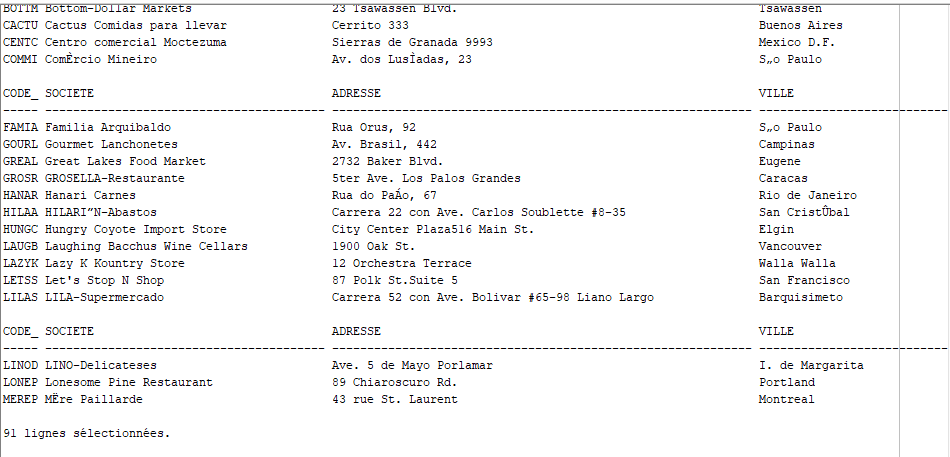
\includegraphics[width=15cm]{EUS_req1.PNG}
    \caption{Première requête : résultat}
\end{figure}

\begin{figure}[!h]
    \centering
    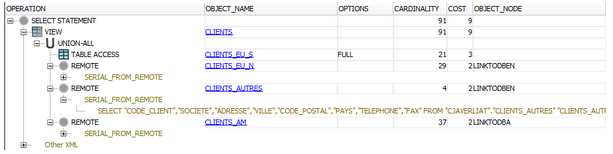
\includegraphics[width=15cm]{EUS_req1_analyse.PNG}
    \caption{Première requête : analyse}
\end{figure}
\newpage

\subsubsection{Deuxième requête}
\inputminted{sql}{EUS_IV-A-2.sql}
\begin{figure}[!h]
    \centering
    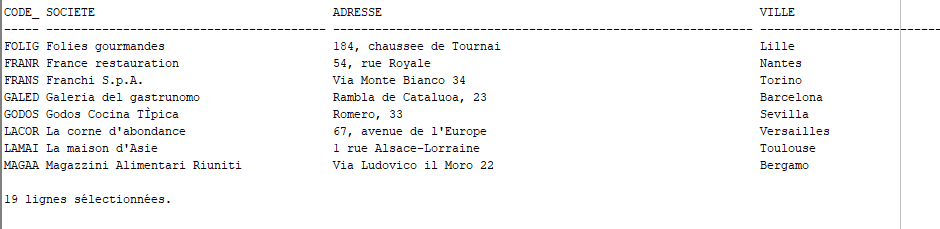
\includegraphics[width=15cm]{EUS_req2.PNG}
    \caption{Deuxième requête : résultat}
\end{figure}

\begin{figure}[!h]
    \centering
    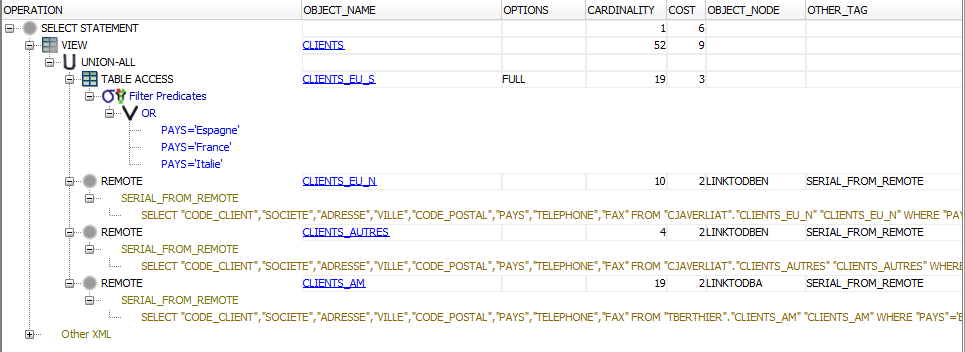
\includegraphics[width=15cm]{EUS_req2_analyse.PNG}
    \caption{Deuxième requête : analyse}
\end{figure}
\newpage

\subsubsection{Troisième requête}
\inputminted{sql}{EUS_IV-A-3.sql}
\begin{figure}[!h]
    \centering
    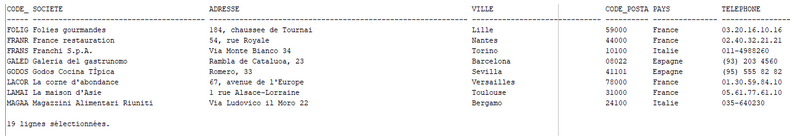
\includegraphics[width=15cm]{EUS_req3.PNG}
    \caption{Troisième requête : résultat}
\end{figure}

\begin{figure}[!h]
    \centering
    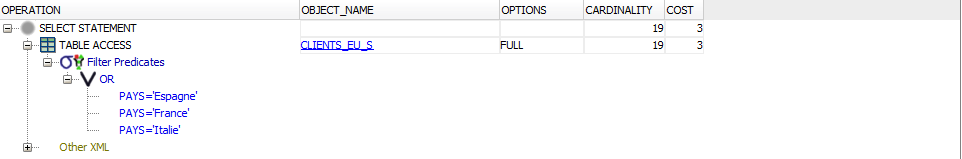
\includegraphics[width=15cm]{EUS_req3_analyse.PNG}
    \caption{Troisième requête : analyse}
\end{figure}
\newpage

\subsubsection{Quatrième requête}
\inputminted{sql}{EUS_IV-A-4.sql}
\begin{figure}[!h]
    \centering
    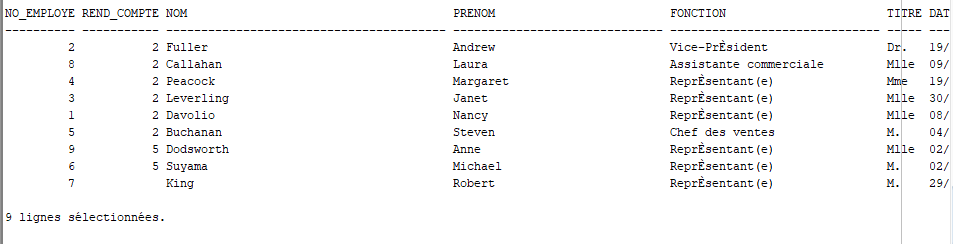
\includegraphics[width=15cm]{EUS_req4.PNG}
    \caption{Quatrième requête : résultat}
\end{figure}

\begin{figure}[!h]
    \centering
    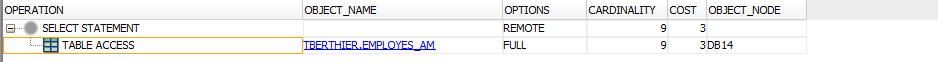
\includegraphics[width=15cm]{EUS_req4_analyse.PNG}
    \caption{Quatrième requête : analyse}
\end{figure}
\newpage

\subsection{Europe du Nord}
%
\newpage

\subsection{Amérique}
%
\newpage

\section{Réplications}
\subsection{Europe du Nord}
Rappel binôme responsable : Charles Javerliat, Pierre Sibut-Bourde \verb|B3109|.
\subsubsection{Objectifs}
%

\subsubsection{Liste des réplications prévues}
Trois réplications vont s'opérer sur ce site :
\begin{itemize}
    \item Employés
    \item Produits
    \item Catégories
\end{itemize}

\subsubsection{Analyse}
%

\subsubsection{Mise en \oe uvre des réplications pour des besoins locaux}
On utilise à ce sujet :
\inputminted{sql}{INSA-DB12-EuropeNord-replication.sql}
Respectivement, on a :
\begin{itemize}
    \item Message émis au site maître : aucune demande
    \item Réponse du site maître : aucune réponse
    \item Tests de vérification de bon fonctionnement de la réplication : on fait un \verb|INSERT| dans la table chez le site maître et l'on vérifie que ce qui est inséré apparaît bien dans la réplication réalisée.
    \item Évolutions éventuelles des contraintes d'intégrité
    \item Évolutions éventuelles des vues et des synonymes
\end{itemize}
~\\
Concernant les réplicats, on a :
\inputminted{sql}{INSA-DB12-EuropeNord-vues-replicats.sql}
Dans tous les cas, on vérifiera la réplication en utilisant \verb|INSERT| et en vérifiant que le tuple inséré est apparent dans le réplicat nouvellement créé.

\newpage

\subsection{Europe du Sud}
Rappel binôme reponsable : OULD HAMOUDA Aymen, LAFAILLE Yann, \verb|B3111|

\subsubsection{Objectifs}
%

\subsubsection{Liste des réplications prévues}
Deux réplications sont prévues pour ce site :
\begin{itemize}
    \item Employés
    \item Fournisseurs
\end{itemize}
Comme les tables Produits et Catégories sont locales, il n'y aura pas de réplication.

\subsubsection{Analyse}
%

\subsubsection{Mise en \oe uvre des réplications pour les besoins locaux}
\textbf{Fournisseurs}
\begin{itemize}
    \item Opéations réalisées localement
    \inputminted{sql}{EUS_V-A-5-a1.sql}
    \item Message émis au site maître : aucune demande
    \item Réponse du site maître : aucune réponse
    \item Tests de vérification de bon fonctionnement de la réplication : on fait un \verb|INSERT| dans la table chez le site maître et l'on vérifie que ce qui est inséré apparaît bien dans la réplication réalisée.
    \item Évolutions éventuelles des contraintes d'intégrité
    \item Évolutions éventuelles des vues et des synonymes
\end{itemize}

\textbf{Employés}
\begin{itemize}
    \item Opéations réalisées localement
    \inputminted{sql}{EUS_V-A-5-b1.sql}
    \item Message émis au site maître : demande de \emph{materialized view log} sur Employés sur le site Amérique
    \item Réponse du site maître : \inputminted{sql}{EUS_V-A-5-b3.sql}
    \item Tests de vérification de bon fonctionnement de la réplication : on fait un \verb|INSERT| dans la table chez le site maître et l'on vérifie que ce qui est inséré apparaît bien dans la réplication réalisée.
    \item Évolutions éventuelles des contraintes d'intégrité
    \item Évolutions éventuelles des vues et des synonymes
\end{itemize}


\end{document}
